%\documentclass[12pt,preprint]{aastex6}
\documentclass[12pt]{article}

\bibliographystyle{aasjournal}

\usepackage{aas_macros} % need this because not using aastex or emulateapj
\usepackage{graphicx}
\usepackage[suffix=]{epstopdf}
\usepackage{natbib}
\usepackage{amsmath}
%\usepackage{url}
\usepackage{xspace}
\usepackage{fullpage}

%    Make Scientific Notation
\providecommand{\e}[1]{\ensuremath{\times 10^{#1}}}

% make the word Kepler italicized
\newcommand{\Kepler}{\textsl{Kepler}\xspace}
\newcommand{\racomment}[1]{{\color{red}#1}}
\newcommand{\ktwosc}{{\tt K2SC}}
\newcommand{\ktwo}{{\tt K2}}
\newcommand{\av}{$A_v$}
\newcommand{\eg}{{\it e.g.}}
\newcommand{\ie}{{\it i.e.}}
\newcommand{\feh}{$[Fe/H]$}
\newcommand{\teff}{$T_{\mathrm{eff}}$}

% fuzzy math
\def\lesssim{\mathrel{\hbox{\rlap{\hbox{\lower3pt\hbox{$\sim$}}}\hbox{\raise2pt\hbox{$<$}}}}}
\def\gtrsim{\mathrel{\hbox{\rlap{\hbox{\lower3pt\hbox{$\sim$}}}\hbox{\raise2pt\hbox{$>$}}}}}

\begin{document}
%%%%%%%%%%%%%%%%%%%%%%

{\bf THIS PAGE INTENTIONALLY BLANK TO LAZILY MAKE PAGE-NUMBERS WORK}
\clearpage


\title{\vspace{-0.5in}Scientific/Technical/Management}
\date{}

\maketitle


% shrink up the space between the "title" and first section heading
\vspace{-1in}

%%%%%%%%%%%%%%%%%%%
\section{Introduction}

%% uhoh, i was about to send up an entire introduction... maybe we should coordinate more about writing sections! :)


Among the key observational properties of main sequence stars in our Galaxy,
age is the most difficult to determine.
Traditionally, fitting isochrones to cluster stars was one of the only precise
methods for measuring ages but was extremely difficult for the majority of
isolated field stars, particularly for those without precise spectroscopic
information.
Methods such as asteroseismology and measuring Lithium abundances can provide
precise ages but require time intensive observations for each target and are
not capable of producing the large quantity of ages needed for exoplanet and
galactic population studies.
To improve our understanding of star and planet formation and evolution, as
well as the history of the Milky Way, we must constrain the ages of
low-mass stars like the Sun in the galactic field.

Fortunately nature has provided a powerful means to determine ages for main
sequence stars via their rotation.
Angular momentum is carried away though magnetically driven stellar winds,
which slows the star's rotation over cosmic time.
This rotation-based ``clock'' is known as {\it gyrochronology}.
Cool spots on the star's surface rotate in-to and out-of view, creating small
amplitude ($\sim$1\%) quasi-periodic changes in the stellar brightness.
While rotation periods have previously been %laboriously
measured from
starspot-induced flux modulations for hundreds of stars from the ground,
space-based photometric surveys have opened the door to homogeneous ensemble
measures of stellar rotation, and therefore age.
{\bf With precise, long-duration light curves available from the \Kepler/K2
mission, we can determine rotation periods and ages for nearly 100,000
main sequence field stars.}
%Stellar rotation periods are are the most promising tool for constraining the
%ages of field stars.

The \Kepler mission broke new ground by producing rotation periods for over
34,000 field stars within a single $\sim$110 sq deg field of view, and
discovered a surprising bimodal distribution of rotation periods
\citep{mcquillan2014}.
Two competing explanations have arisen for this mysterious feature: a bimodal
age distribution for nearby stars, or a new subtlety in stellar
angular-momentum-loss mechanisms.
Detailed calibrations of gyrochronology models with the \Kepler rotation
sample also revealed the need for samples of stars with a wider range of ages
and compositions.
Fortunately the ongoing \Kepler extended mission, K2, has currently produced
light curves from 14 additional fields throughout the Galaxy.

To enable studies of stellar ages from rotation periods with K2, we propose
to:

{\bf 1.} Measure accurate rotation periods for every available K2 target,
using the most appropriate tools and methods required.
% using new statistical methods we have developed to cope with significant
% instrumental systematics in the K2 data.
This value-added dataset will improve the \Kepler data legacy for field stars,
and provide a critical training set for the TESS mission.

{\bf 2.} Produce updated gyrochronology relations based on a wider range of
field star ages, and additional open clusters within the K2 fields.
% mention homogeneity of field and cluster sample?

{\bf 3.} Determine the origin of the mysterious rotation period bimodality
discovered with \Kepler by tracing the rotation period distribution in each K2
field, and out to further distances utilizing public Gaia data.

{\bf 4.} Measure the star formation history within each K2 field using a new
Bayesian age-dating system.



\clearpage



%%%%%%%%%%%%%%%%%%%
\section{Scientific Motivation}
Galactic archaeology and exoplanet populations are two rapidly accelerating
fields of interest within astronomy.
Although seemingly unconnected, these two fields are linked by a mutual
requirement for precise stellar parameters.
To galactic archaeologists, ages and elemental abundances are the most
important parameters.
Indeed, most galactic archaeology surveys target exactly these properties.
For exoplaneteers, masses and radii have historically been the most important
stellar parameters for understanding planetary systems.
With a growing number of planet hosts with precise masses and radii, attention
is turning toward other parameters such as ages to understand the history and
evolution of these systems.
Age is therefore a fundamental stellar parameter of great interest to two
large communities of astronomers.
However it is a difficult attribute to measure for main sequence F, G, K, and
M stars in the field, in part because low-mass dwarfs do not move far on the
Color-Magnitude diagram (CMD) during their hydrogen burning lifetimes.
Further, competing stellar evolution models predict different ages for the
same star.
%Asteroseismology, while a very precise age-dating tool, is not capable of
%producing the large quantity of ages needed for exoplanet and galactic
%population studies.
Of the measurable properties for a large ensemble of field stars, rotation
periods contain the most information about stellar age, and provide the best
leverage for advancing our knowledge of galactic archeology as well as
exoplanet population demographics.


%%%%%%%%%
\subsection{Age-Dating Field Stars with Rotation}
The seminal work of \citet{skumanich1972} laid the foundation for our model of
the stellar age--rotation--activity relationship.
When stars settle onto the main sequence they may have a range of initial
rotation periods based on the angular momentum available in their primordial
environment.
However, rotation velocities for Solar-type stars converge after around 500 Myr \citep{radick1987,irwin2009b}, and then follow a standard spin-down
evolution \citep{barnes2010}.
Main sequence stars continuously lose angular momentum due to
magnetically driven winds \citep{schatzman1962, weber1967, mestel1984,
kawaler1988, charbonneau2010}.
Since stellar rotation also drives the internal magnetic dynamo
\citep[][]{schatzman1962, parker1970}, the result of this angular momentum
loss is decreasing surface magnetic activity as the star slows.
Older, slower rotating stars therefore have smaller starspots, making the
detection of their rotation more difficult as stars age.
This rate of angular momentum loss has a dependence on the stellar mass
\citep{noyes1984}.
Deriving ages for field stars therefore requires knowing their color (as a
proxy for stellar mass) and their present-day surface rotation period
\citep{barnes2007}.
% These gyrochronology estimates can produce ages with errors as low as
% $\sim$10\% \citep{barnes2010}.

The rate of this angular momentum loss has historically been calibrated using
main sequence stars at a range of masses in stellar clusters with known ages,
leading to a useful clock called ``gyrochronology'' \citep{barnes2003}.
Several gyrochronology model parameterizations exist, each using various age
benchmarks for calibration \citep[\eg][]{barnes2007, barnes2010, mamajek2008,angus2015, Matt2012, van-saders2013, van-saders2016}.
Nearly all gyrochronology models suffer from lack of constraints at older
ages; often the Sun is the only benchmark used older than $\sim$1 Gyr since
accessible nearby open clusters are typically young ($<600$ Myr).

\begin{figure}[!t]
\centering
% 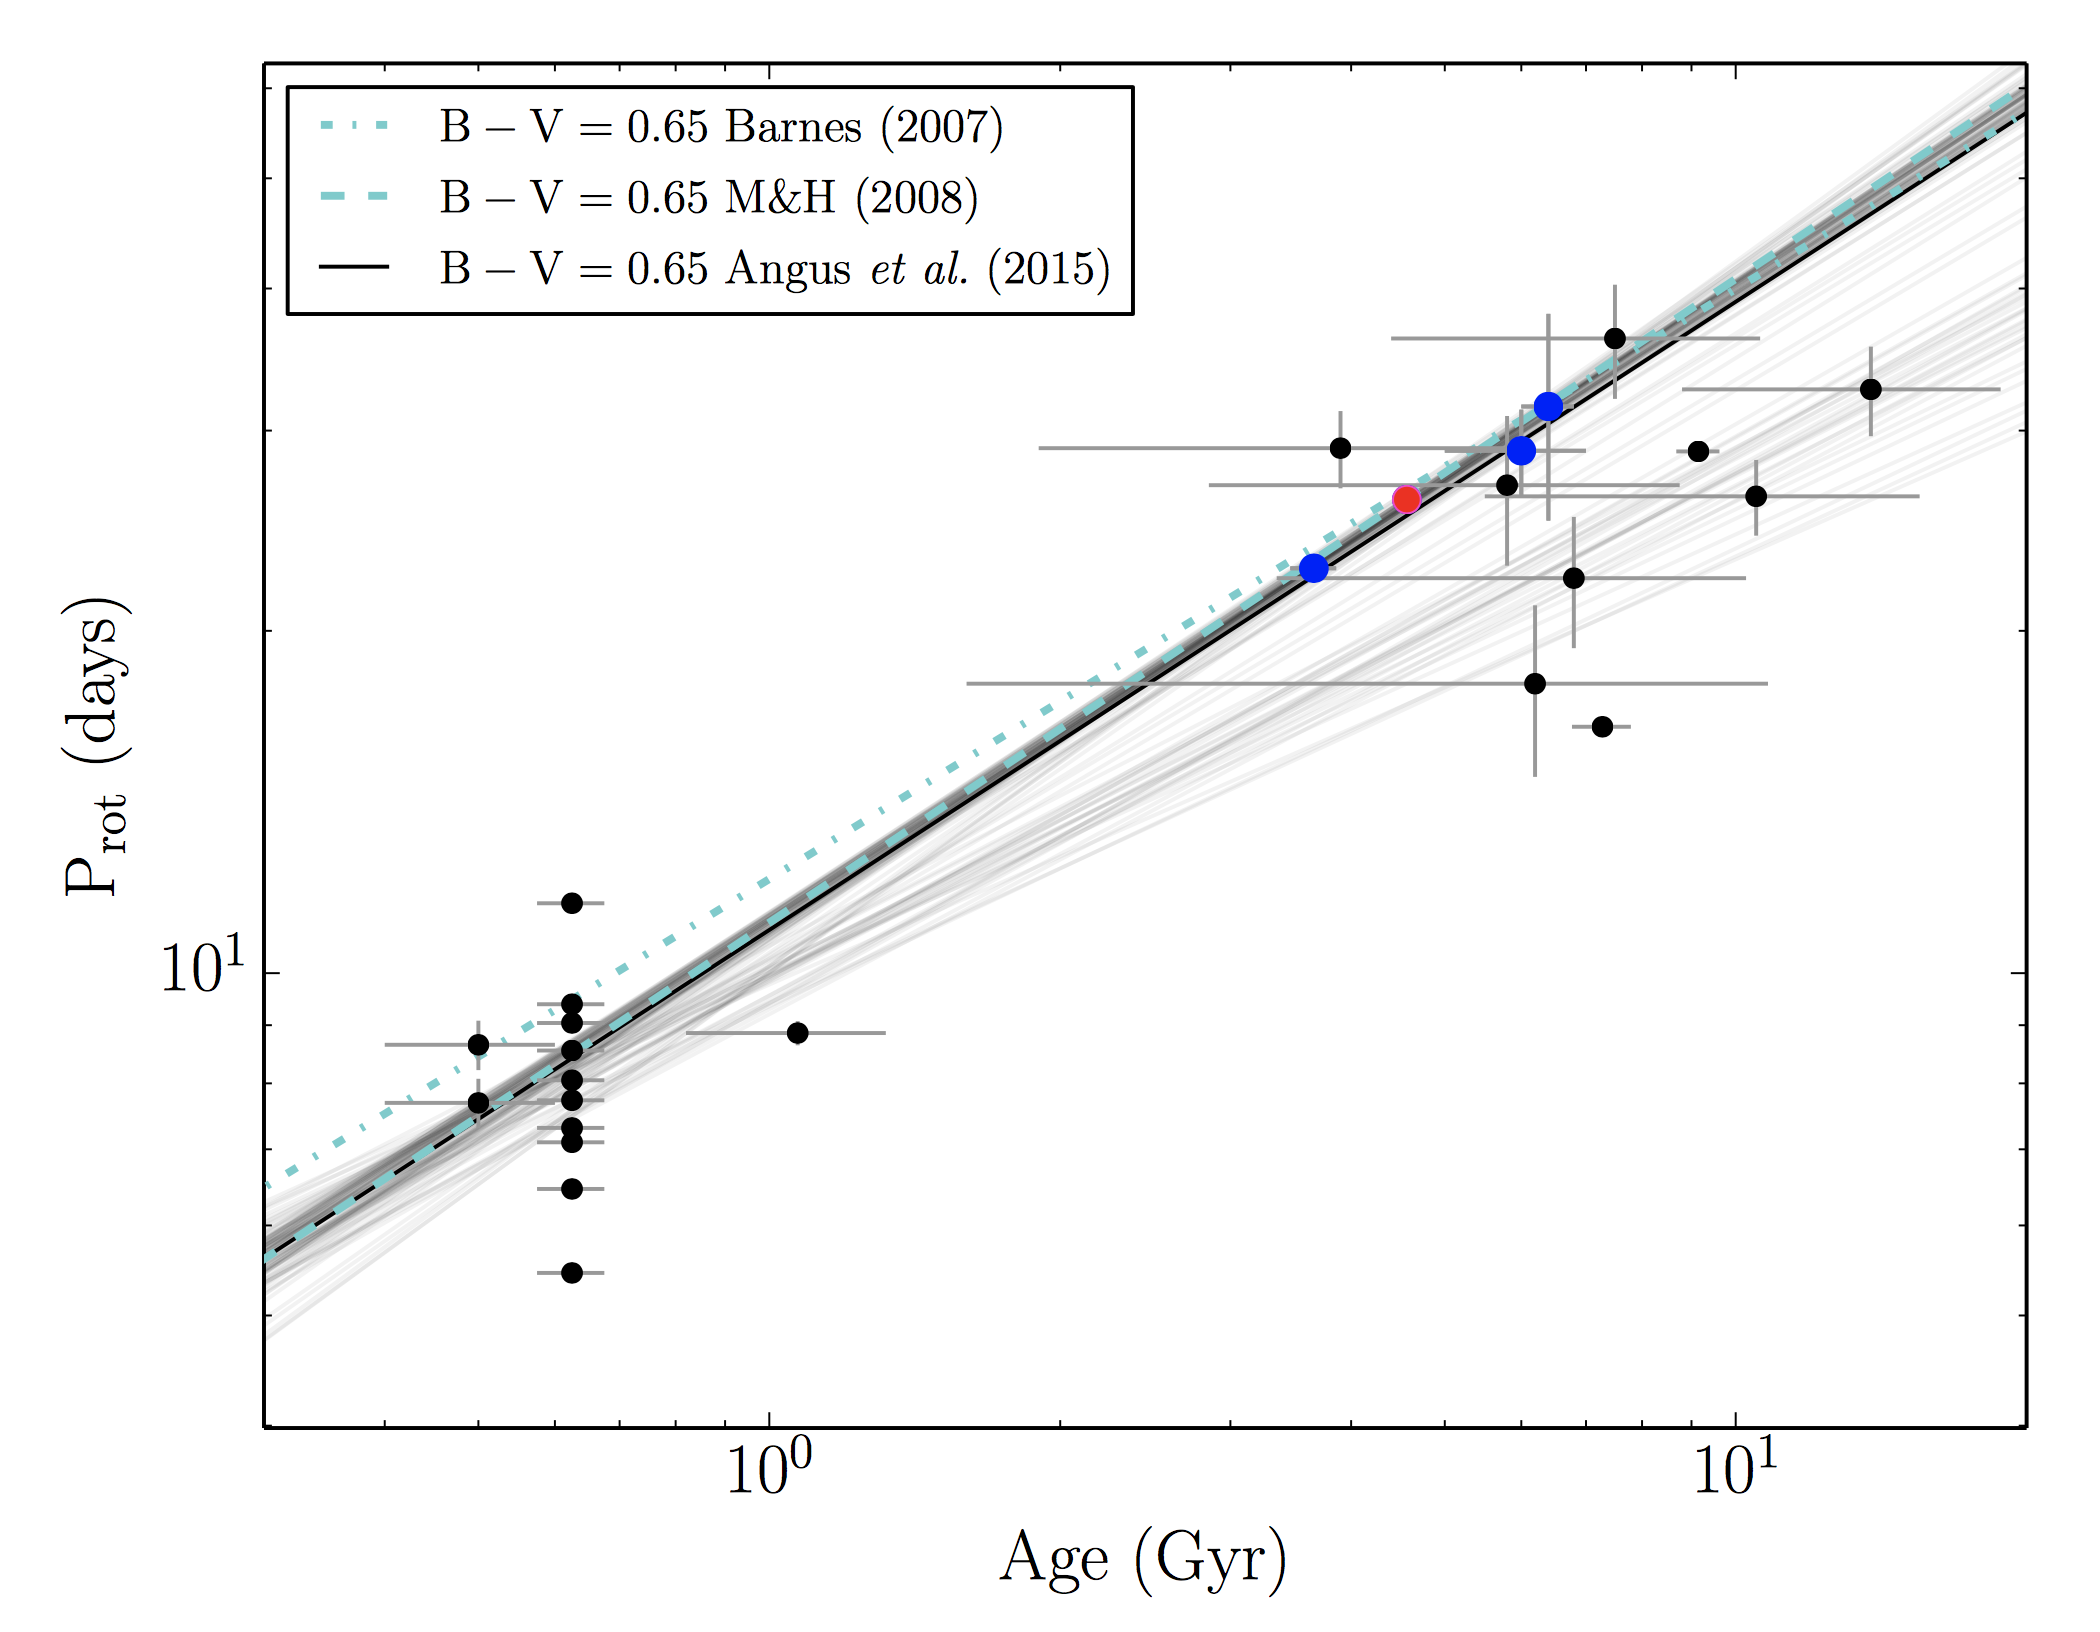
\includegraphics[width=4in]{angus2015_fig6.png}
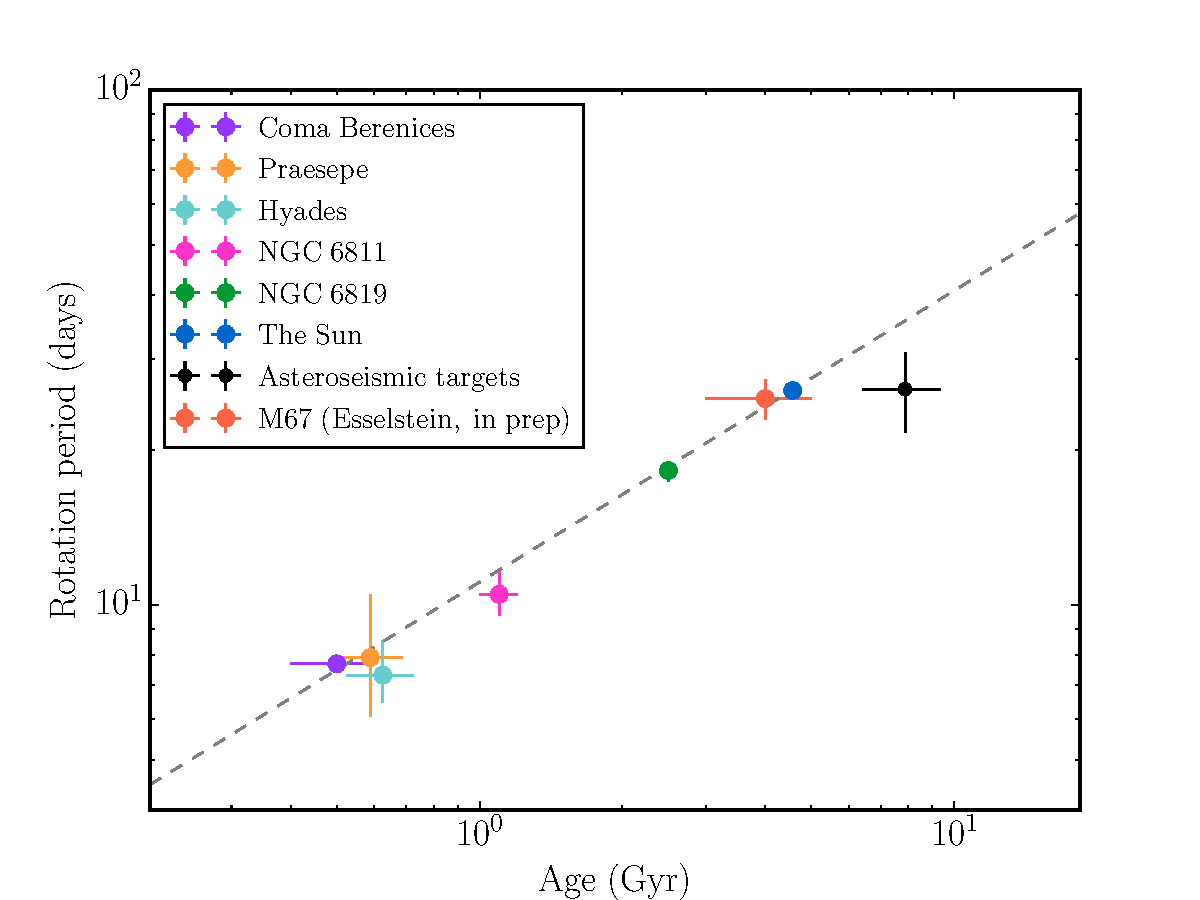
\includegraphics[width=4in]{AAS_talk_M67_astero.pdf}
    \caption{A gyrochronology relation (dashed grey line) demonstrating the
    rotational evolution of stars with precise ages.
    Median rotation periods for Solar-type stars in open clusters (colored points), Solar mass \Kepler asteroseismic targets (black point), and the Sun (blue point).
%    Each colored point (except the dark blue point) represents the median
%    rotation period for Solar-type stars in open clusters as indicated in the legend.
%    The blue point represents the Sun and the black point is the median
%    rotation period and age for main sequence, Solar-color \Kepler
%    asteroseismic targets.
    The black point falls below the straight line, indicating that there may
    be a transition in age-rotation relation at around Solar age.}
\label{fig:gyro}
\end{figure}

In Figure \ref{fig:gyro} we demonstrate the discrepancy between a single
power-law gyrochronology model and the most recent asteroseismic data from
the \Kepler sample.
As first demonstrated in \citet{angus2015}, the asteroseismic stars seem to be
too rapidly rotating given their age, according to the gyrochronology models.
This finding was supported by \citet{van-saders2016} who used \Kepler
asteroseismic targets to redefine the gyrochronology models.
To explain this phenomenon \citet{van-saders2016} invoke a transitioning magnetic dynamo
behavior at a critical Rossby number, $Ro$\footnote{The Rossby number is the
ratio of rotation period to convective overturn time.} which they find to be
$Ro\approx2.7$ (close to the Solar value).
This transition marks a boundary between efficient magnetic braking (2.7 $<$
$Ro$) to inefficient braking ($Ro$ $<$ 2.7); stars stop spinning down after
their rotation slows enough to cross this critical threshold.
{\bf This has extremely important consequences for gyrochronology: can we trust
ages inferred from rotation for slowly rotating stars like the Sun?}

Additional calibration sources are desperately needed for stars older than the
Sun in order to confirm these hints of a changing angular momentum loss rate due to a transitioning magnetic dynamo.
Asteroseismology also cannot yet provide ages for stars with masses
much lower than the Sun, leading to an incomplete calibration of the gyrochronology models.
\citet{douglas2017} used \ktwo observations of the Hyades to demonstrate that
gyrochronology may be applicable to stars with masses as low as 0.3 $M_\odot$. While rotation periods of many more low-mass stars are needed to confirm this exciting finding, if confirmed it would be an important result for exoplanet studies,
which have increased focus on M dwarfs due to the higher signal-to-noise of planet characterization provided by the smaller stellar radii and masses.
%If it is confirmed that gyrochronology is applicable to these low-mass stars,
%it will be possible to infer the ages of the planets orbiting them.

% \citet{Metcalfe2017} went on to use these same data, the main sequence \kepler
% asteroseismic targets, to demonstrate that the Solar magnetic dynamo may be
% in transition.

% \Kepler rotation period samples have demonstrated that magnetic braking may
% become less efficient at older ages \citep{van-saders2016}.
% The \citet{angus2015} gyrochronology study also found that cluster and
% asterosismic field star targets may not follow the same spin-down model,
% possibly indicating bias in the dynamical histories of these samples.

%%%%%%%%%
\subsection{Rotation Periods from \Kepler and K2}
Previous ground-based efforts to constrain stellar rotation periods for single, isolated field stars have resulted in few measurements. Detecting rotation from Doppler line broadening requires obtaining medium- to high-resolution spectroscopy of individual targets, and can be subject to systematic effects such as from stellar limb darkening approximations \citep{collins1995}. These observations also require time on larger aperture telescopes to reach fainter magnitudes needed to study rotation from low-mass field stars, or for studying the entire mass range within stellar clusters. Ground-based photometric wide-field surveys overcome many of the difficulties in gather large samples of field stars or entire stellar clusters. However, long duration monitoring with relatively high cadence and high photometric precision is required to detect the small amplitude and slowly varying flux modulations from starspots. These campaigns typically yielded rotation samples of hundreds to $\sim$1000 for both field stars \citep[e.g.][]{hartman2011} and selected young open clusters \citep[e.g.][]{agueros2011,douglas2014,covey2016}


Space-based photometry surveys designed for exoplanet transit searches such as \Kepler \citep{borucki2010} have produced a revolution in stellar rotation studies. The original \Kepler mission produced light curves up to four years in duration with $\sim$100 ppm precision at 30-minute cadence for more than 200,000 stars. From this remarkable dataset, more than 30,000 unique stellar rotation periods have been measured using a variety of time series analysis techniques such as the Lomb-Scargle Periodogram \citep{reinhold2013} and the Autocorrelation Function \citep[][]{mcquillan2014}.
This bounty of rotation periods has also allowed the first ensemble investigations into stellar surface differential rotation \citep[e.g.][]{reinhold2013}, revealed stars with near solid-body rotation \citep{davenport2015a}, and highlighted the many degeneracies in disentangling starspot evolution and differential rotation \citep{aigrain2015}.


After hardware failures made observations of the original field impossible, an extended \Kepler mission was designed to observe many fields with $\sim$3 month durations. The K2 mission has observed fields spaced along the ecliptic plane, ranging from low galactic latitudes that include multiple open clusters, to high galactic latitudes that include many older field stars \citep{howell2014}. The K2 fields also include several benchmark stellar clusters including the Solar-age M67, the Pleiades and Hyades, and M35. To date K2 has released data from 10 distinct campaigns (or fields), including more than 204,000 targets. An additional 4 campaigns are underway with $\sim$94,000 targets announced, and 2 campaigns pending scheduling. In total, the K2 sample may yield over 350,000 light curves, far exceeding the original \Kepler mission. Importantly, K2 data quality has been demonstrated to approach that of the original \Kepler mission \citep{luger2016}, and has been successfully used to measure rotation periods for select targets such as open cluster stars \citep[e.g.][]{douglas2017}.


\clearpage % added to prevent half of first sentence from being on previous page - remove if major edits above!
{\bf K2 provides the ideal dataset to both extend the \Kepler studies of field star age distributions, and to amass a sample of better calibration sources for gyrochronology models.} The range of K2 field positions within the Galaxy means the sample spans a much wider variety of stellar ages for more distant stars ($\gtrsim$1pc), and provides multiple opportunities to constrain the local star formation history for nearby stars. This makes the gyrochronology study of field stars with K2 an unique and valuable comparison to complimentary efforts in studying galactic archeology using chemical abundances, such as with APOGEE \citep{hayden2014}.
Producing rotation periods for these older stars and additional open clusters available in the K2 data, including the benchmark Solar-age cluster M67, will also lead to new gyrochronology relations and to test the universality of the age--rotation--activity relation put into question by \citet{angus2015}.



%%%%%%%%%
\subsection{A Mysterious Period Bimodality}

One of the most remarkable results from the \Kepler rotation period catalog was the discovery of a bimodal period distribution among field stars by \citet{mcquillan2013}, which is shown in Figure \ref{fig:bimodal}a. While a separate sequence of rapid rotation periods had been known in young stellar clusters due to lower-mass stars settling on to the angular momentum main sequence slower \citep[e.g.][]{barnes2007}, this new bimodality was detected from slower rotating M dwarfs ($T_{eff}\lesssim4000$). The bimodality separated M dwarfs into two populations, those with rotation periods longer than $\sim$20 days, and those with periods between $\sim$1 and 20 days. Follow-up analysis of the \Kepler data by \citet{mcquillan2014} found the period bimodality extended to include K dwarfs. {\bf Recently, PI Davenport discovered this period bimodality extends throughout all masses in the \Kepler rotation sample for nearby stars, as shown in Figure \ref{fig:bimodal}b \citep{davenport2017}.}

\begin{figure}[!th]
\centering
\makebox[\textwidth][c]{ % sloppy hack to make figure slightly overflow
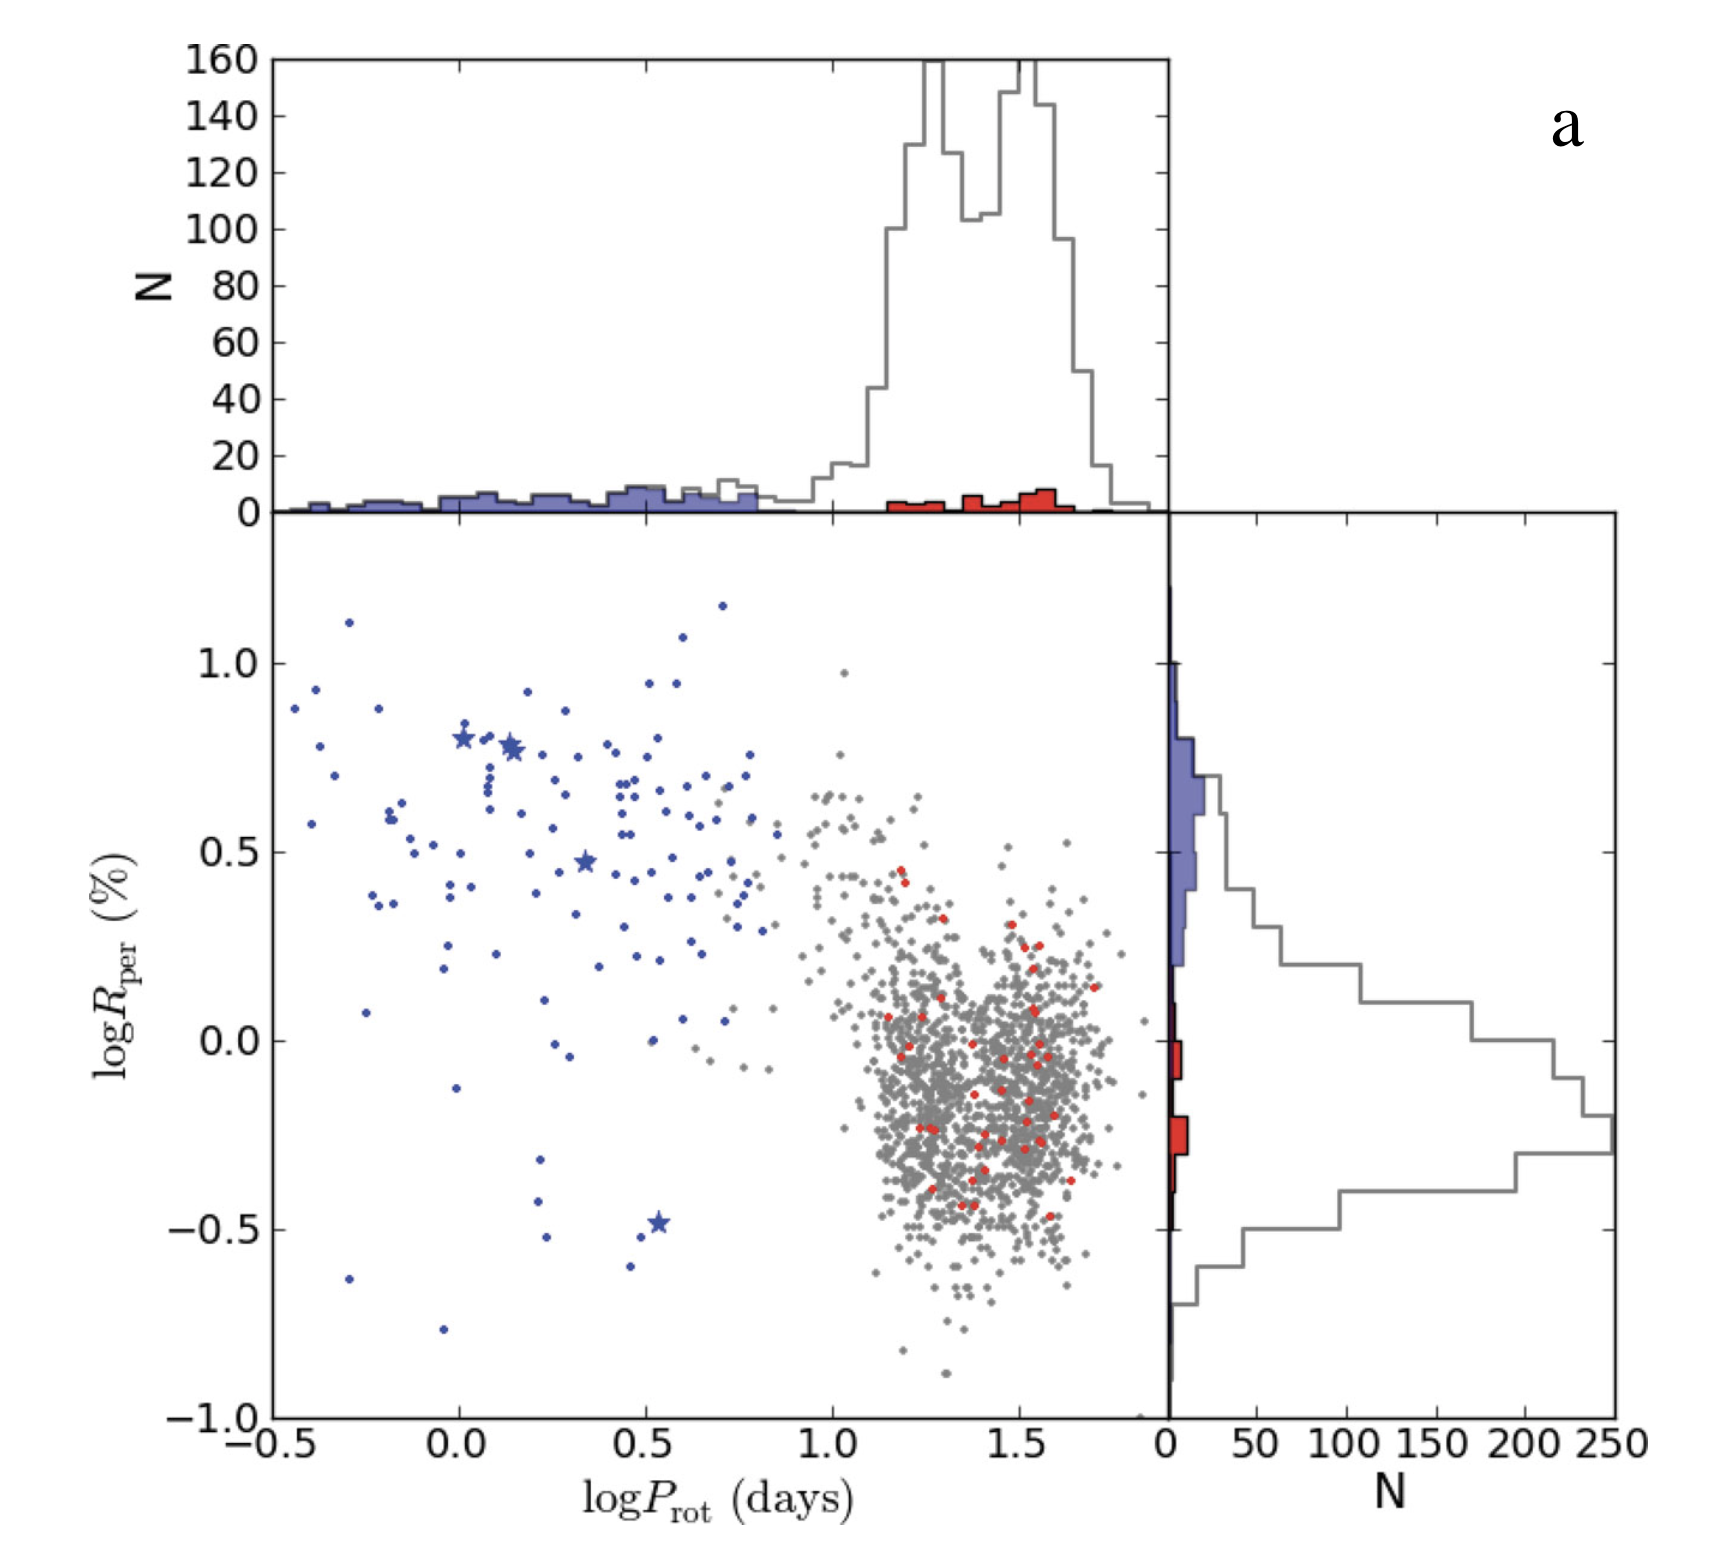
\includegraphics[width=3in]{mcquillan2013_fig9.png}
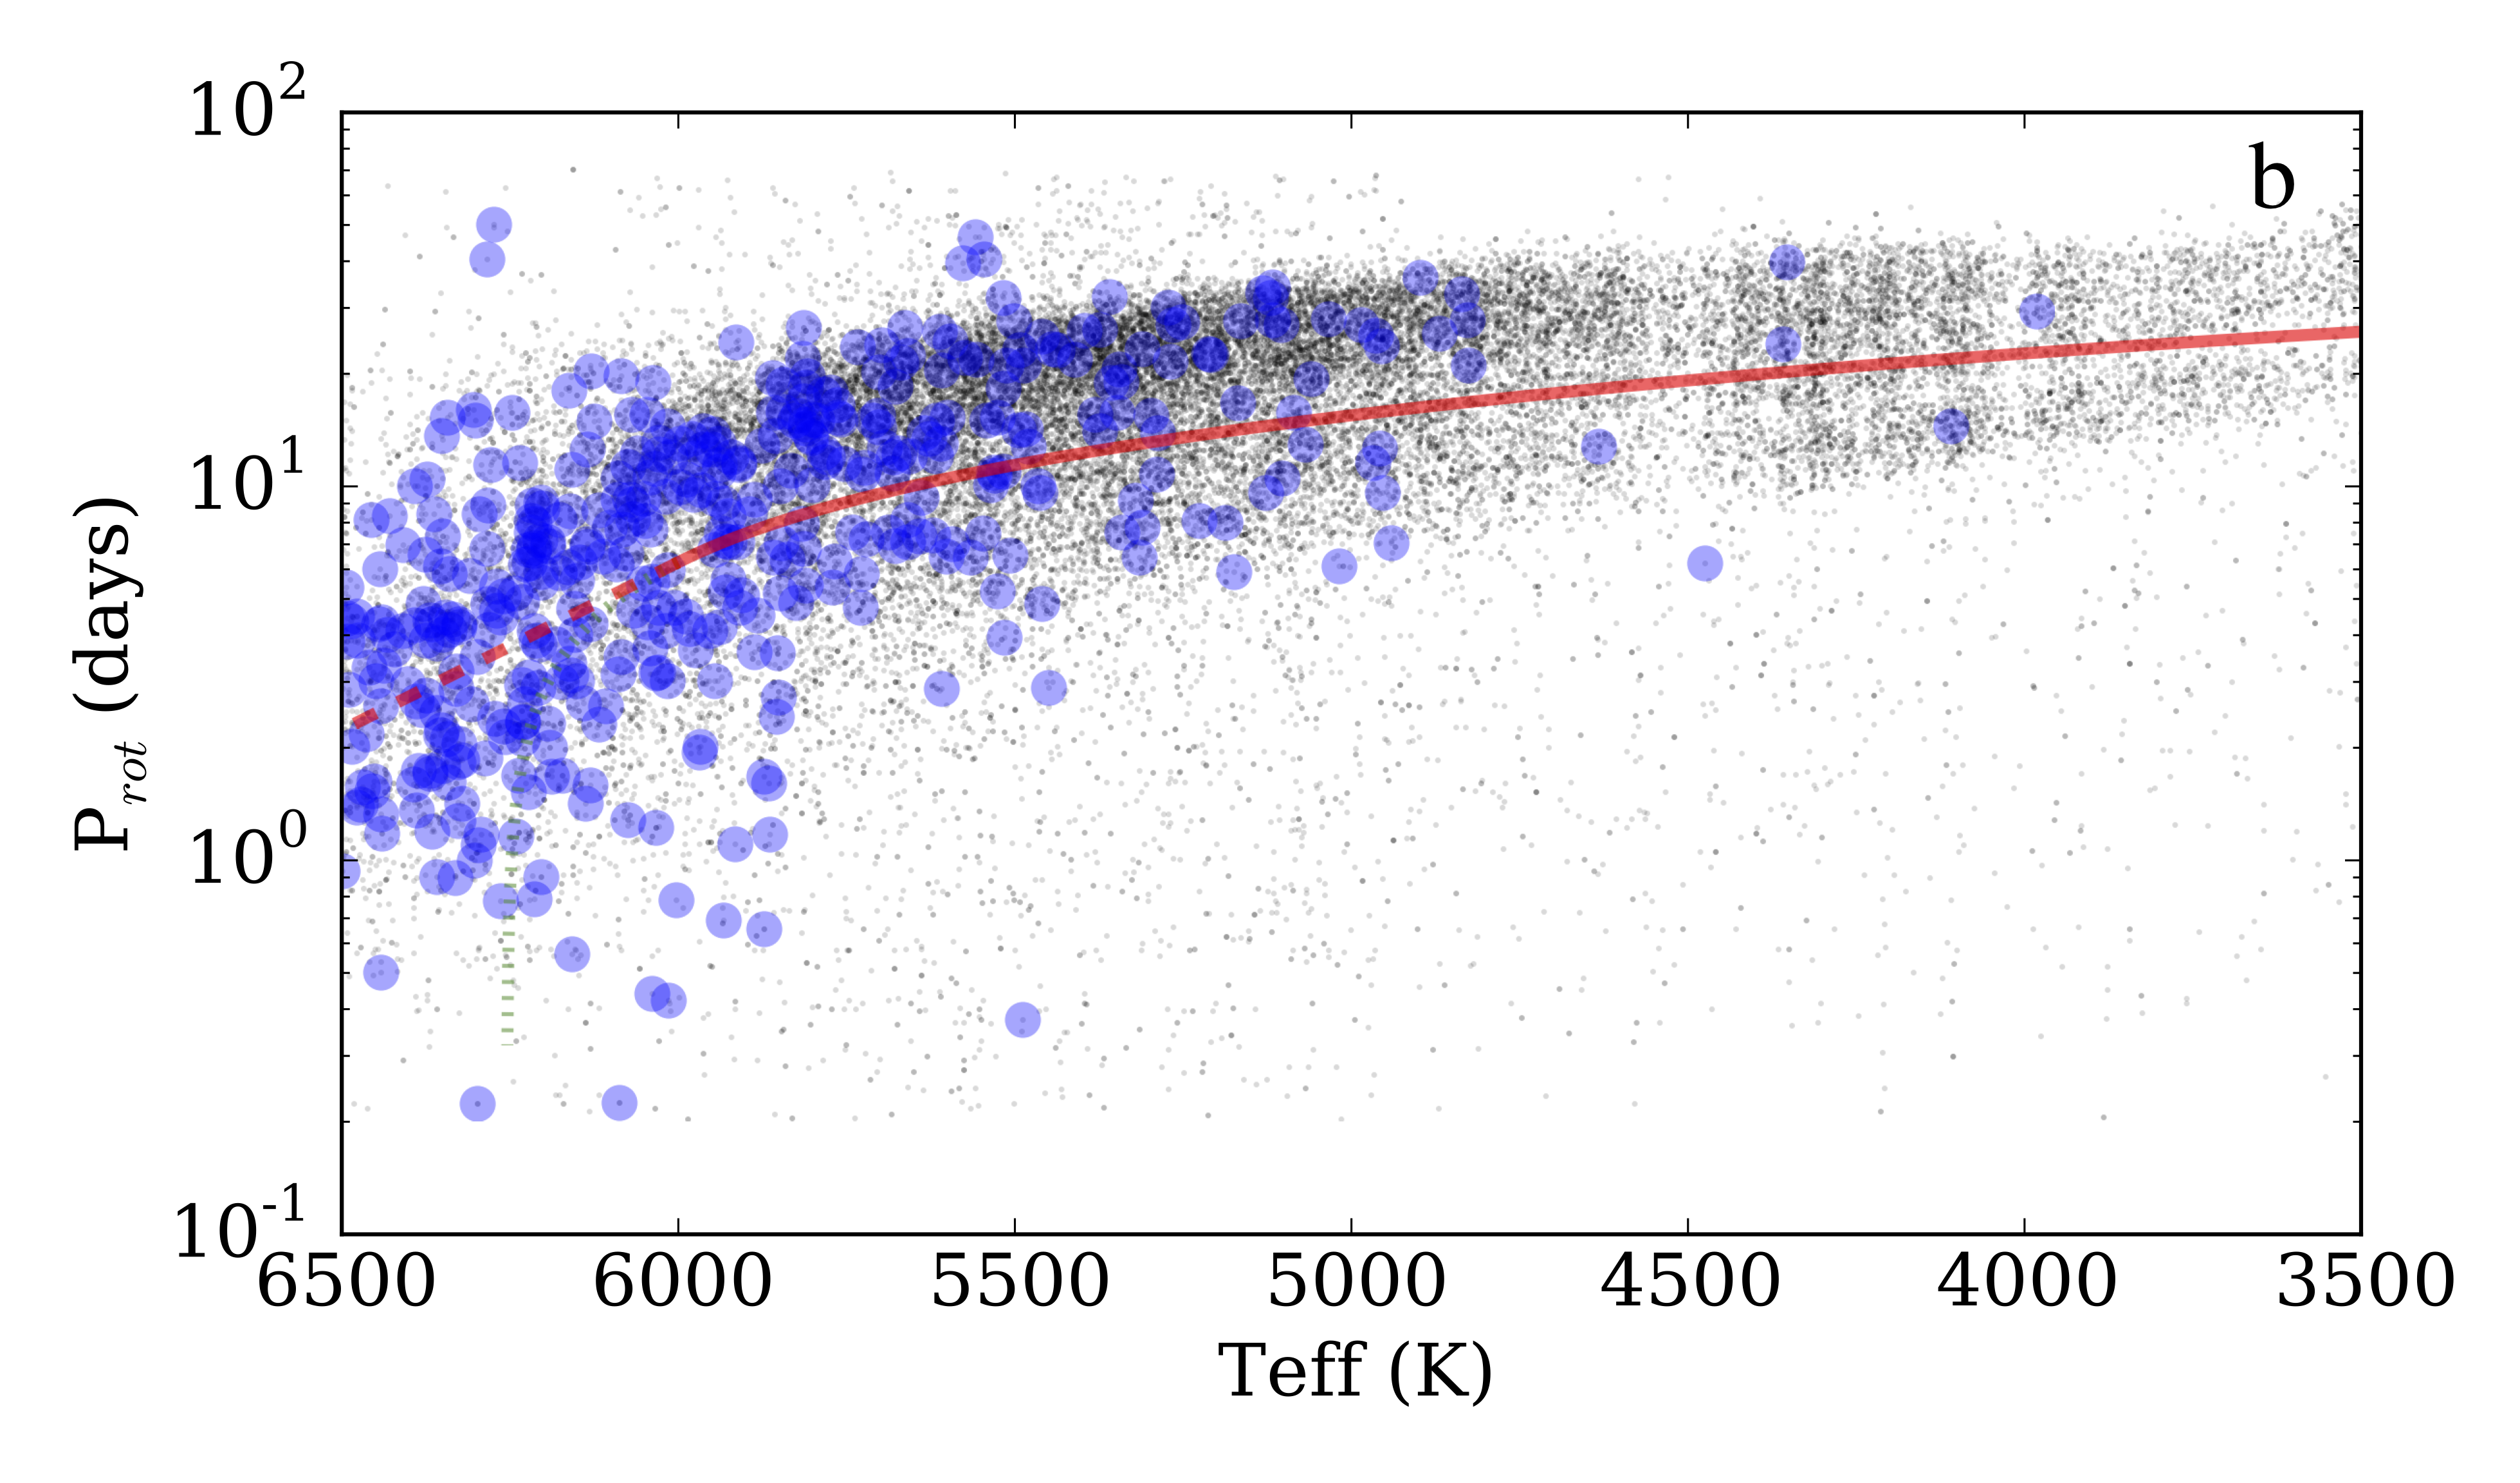
\includegraphics[width=4in]{davenport2016_fig3.png}
}
\caption{
Left -- Figure 9 from \citet{mcquillan2013}; the discovery of a bimodality in rotation periods from \Kepler M dwarfs (middle panel).
Right -- Figure 3 from \citet{davenport2017}, showing all \Kepler rotation periods from \citet{mcquillan2014} (black dots), and main sequence stars with Gaia DR1 distances (blue circles). The bimodality discovered for M dwarfs extends to nearby G and K stars, and straddles a 600 Myr ``gyrochrone'' (red line).
}
\label{fig:bimodal}
\end{figure}




{\bf Two formation scenarios have been proposed to explain the observed period bimodality.} The first scenario, initially proposed by \citet{mcquillan2013}, is the rotation period distribution reflects the local star formation history, and thus the bimodality represents a drop in the star formation rate around 600 Myr ago. This model is supported by both the extension of the bimodality to earlier spectral types by \citet{davenport2017}, and also the tentative detection that the two rotation period populations have distinct proper motion distributions. However, such a variation in the star formation rate on short timescales has some tension with independent observational efforts to determine the local star formation history. While Color--Magnitude diagram inversions from Hipparcos have suggested a similarly short timescale variation in star formation of  $\sim$0.5 Gyr \citep{hernandez2000}, other studies find slower variations over several Gyr \citep[e.g.][]{cignoni2006}. Using white dwarf cooling models to infer the local formation history (``cosmochronology'') also supports higher star formation several Gyr ago, but can rarely achieve age resolution better than $\sim$1 Gyr due to small sample sizes \citep{tremblay2014}. The spatial extent of such coherent and localized variations in star formation history is unknown.


The second scenario to explain this feature is that the period bimodality occurs due to a previously unknown variation in the spin-down evolution for low-mass stars. In this model the star formation history would be continuous over the past $\sim$1 Gyr, and around 600 Myr stars would move quickly through the observed period minima due to this unknown phase transition or feedback mechanism. While this model is not predicted by angular momentum loss prescriptions, rapid transitions in rotation period are observed for stars in young clusters. Stars move quickly from the rapidly rotating ``convective'' sequence (periods of $\lesssim1$ day) to the ``interface'' sequence (periods of several days) during the first few hundred Myr, with lower mass stars taking longer to make this transition as they settle onto the main sequence \citep{barnes2003}. Secondly, a gap in chromospheric activity levels for solar-type field stars has also been observed \citep{vaughan1980}. While this magnetic activity indicator smoothly varies with stellar ages over long timescales, the gap indicates a rapid transition phase from ``active'' to ``inactive'' is present within the first Gyr \citep{pace2009}. Thirdly, the angular momentum loss underpinning gyrochronology seems to slow for stars older than the Sun, indicating a potential change in the magnetic dynamo for slower rotators \citep{angus2015,van-saders2016}.


{\bf The K2 rotation period sample provides the ideal dataset to test these two formation scenarios.} If the bimodality is due to an age distribution we would expect to only see the feature locally, and that it could disappear at further distances or along different lines of sight where small scale variations in the star formation history are less apparent. Coherent changes in the rotation period (or stellar age) distribution along opposing Galactic lines of sight might also reveal details of the spiral arm pattern speed near the Sun. The kinematic separation between the two rotation period populations would be reinforced by supplemental measurements from the upcoming public Gaia data releases. However, if the bimodality is truly due to a transition point in the spin-down evolution at young ages, we would expect to find no little to no variation in this feature as seen in Figure \ref{fig:bimodal}b with galactic position, distance, or between K2 fields.





%%%%%%%%%%%%%%%%%%%
\section{Proposed Research}
%%%%%%%%%
\subsection{Measuring Rotation Periods}
We propose the first systematic study of stellar rotation periods from the K2
data. This will include the nearly 300,000 light curves from Campaigns 0-14.


Part of our study will be to assess the qualities of the various data
reduction pipelines available for K2 light curves.
Each detrending algorithm uses a slightly different approach and will almost
certainly provide light curves that differ enough to produce a number of
discrepant rotation periods.
We will compare the performance of three pipelines in particular: the
\citet{Vanderburg2015} light curves, the {\tt everest} \citet{luger2016} light
curves, and the \ktwosc\ \citet{aigrain2016} light curves.
By visually examining the light curves and Lomb-Scargle periodograms of a
number of targets in common between the detrending methods, we will ascertain
which pipeline best preserves signal on long timescales.
% The \ktwosc\ pipeline removes instrumental systematics using a non-parametric
% approach: a Gaussian process is used to model the instrumental systematics,
% astrophysical variability and white noise in each light curve.
% All three of these pipelines are optimized for planet search, however the
% \citet{aigrain2016} light curves are designed to preserve stellar variability
% as much as possible.
% We expect to find that these light curves preserve rotation signals on the
% longest timescales.

Once establishing the best detrending method for preserving stellar
variability, we will download all the available light curves and, if
necessary, run the pipeline on any outstanding targets.
We will also produce and examine periodograms using the
systematics-insensitive periodogram (SIP) \citep{angus2015}.
This method simultaneously fits light curves with a sinusoid and a noise
model constructed from 150 principle components derived from a PCA of the
entire set of \ktwo\ light curves for a given campaign.
Although developed for asteroseismology, this algorithm may also be applicable
to rotation period analysis, however at the longer timescales of variation
produced by stellar rotation, it is likely that the results will suffer from
overfitting and will revert to standard Lomb-Scargle periodogram methods in
this case.

We will use a combination of Lomb-Scargle and autocorrelation function
techniques to produce a quick catalogue for early analysis.
Although both of these methods are sensitive to noise and can produce spurious
rotation period measurements, there relative speed will allow us to rapidly
begin initial analysis of the results.
We will then apply a procedure for obtaining more accurate and precise
rotation periods using probabilistic inference.
Co-I Angus recently developed a method for rotation period inference using a
Gaussian Process (GP) to model the light curve in the time-domain, rather than
extracting periodic signals in the frequency domain \citet{angus2016c}.
% Is this IAU reference correct, or do you have a paper?%\citet{Angus2017}.
This GP method produces slightly more precise and accurate rotation periods
with more representative uncertainties than Lomb-Scargle and autocorrelation
methods.
The disadvantage of this GP regression based method is that it can be
computationally expensive.
However, with the recently developed method for fast Gaussian process
inference, {\tt celerite} \citep{foreman-mackey2017}, even performing MCMC
with the thousands of data points in a \ktwo\ light curve may only take a few
minutes.
The advantage of computing probabilistic rotation periods is that one can
bypass the need to calculate a rotation period at all and simply infer the
parameters of stellar populations directly from the light curves themselves.
In other words, one can perform hierarchical inference more easily.
This may be a level of sophistication that is above and beyond our science
goals but it is worth noting that we could take this approach if the data and
scientific question warranted it.

Wherever possible we will mask out discontinuous astrophysical signals, such as
eclipsing binaries, planet transit or flares that may distort the rotation
period signal.
We will make use of exoplanet and binary catalogs to identify planet transits
and eclipses.
We will apply the flare detection algorithm {\tt appaloosa}, built by PI
Davenport, to identify and remove flares.
It may still be necessary to apply a low-pass filter to the data in order to
remove high frequency features that we miss.
Fortunately, most of the stellar rotation signals of interest for this study
have timescales longer than around a day and will be relatively unaffected by
a low-pass filtering algorithm.

% The \Kepler rotation period catalog from \citet{mcquillan2014} found a yield
% of $\sim25\%$ of stars had measurable rotation periods using the
% Autocorrelation Function.
From our sample of nearly 300,000 available K2 targets, we expect to recover
over 70,000 new periods, bringing the total \Kepler/K2 sample to $\sim$100,000
stars with measured rotation periods.

We have already measured a number of K2 rotation periods using a simple
autocorrelation function approach.
Figure \ref{fig:kalesalad} shows stars observed by K2 during campaign 4,
plotted according to their RA and dec and colored by their rotation period.
To measure the rotation periods shown here we downloaded a
{\tt everest} \citep{luger2016} light curve for every star and computed an
autocorrelation function (ACF) of each light curve.
We smoothed the ACFs and adopted the lag of the highest peak as the dominant
period in the time series.
Due to the simplicity of the period extraction technique and the fact that we
have taken each period measurement at face value with no attempt to remove
astrophysical contaminants, figure \ref{fig:kalesalad} is a {\it very}
preliminary look at rotation and other stellar variability in one of the K2
fields.

\begin{figure}[!th]
\centering
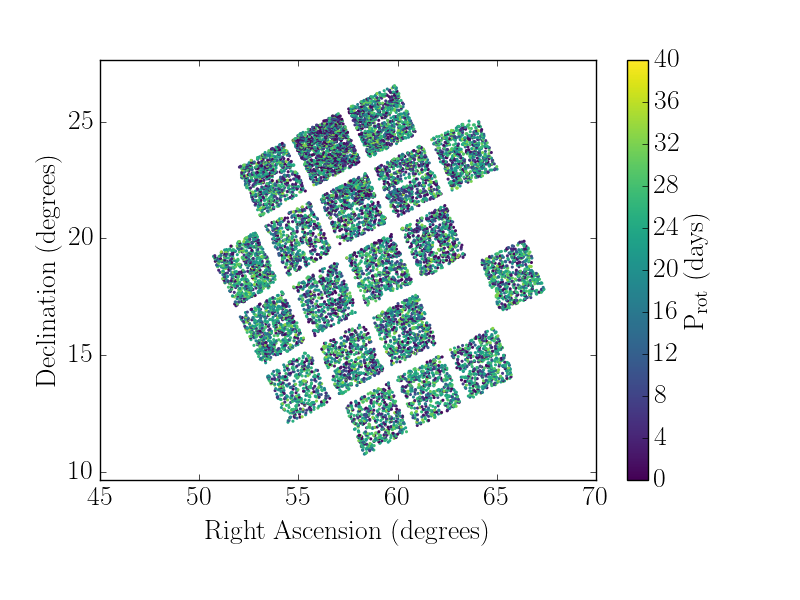
\includegraphics[width=4in]{ra_vs_dec_period_c04.png}
\caption{All stars observed during K2 campaign 4, plotted according to their
    equatorial coordinates and colored by their preliminary rotation period.
These rotation periods were measured using a very simple ACF method, applied
    to {\tt everest} \citep{luger2015} light curves.}
\label{fig:kalesalad}
\end{figure}





%%%%%%%%%
\subsection{Exploring the Period Bimodality}

\begin{figure}[!th]
\centering
\makebox[\textwidth][c]{ % sloppy hack to make figure slightly overflow
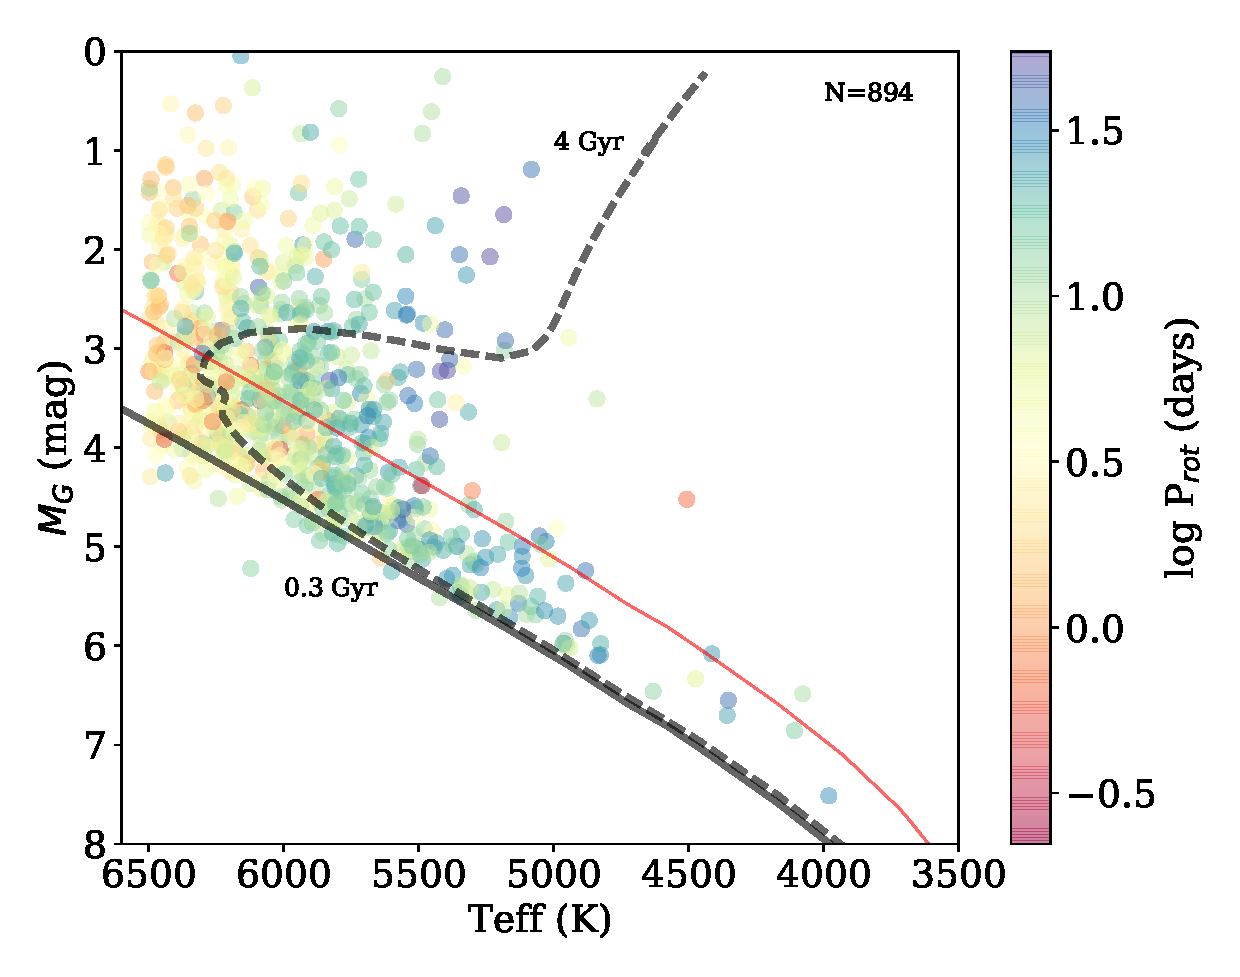
\includegraphics[width=3.5in]{davenport2016_fig2}
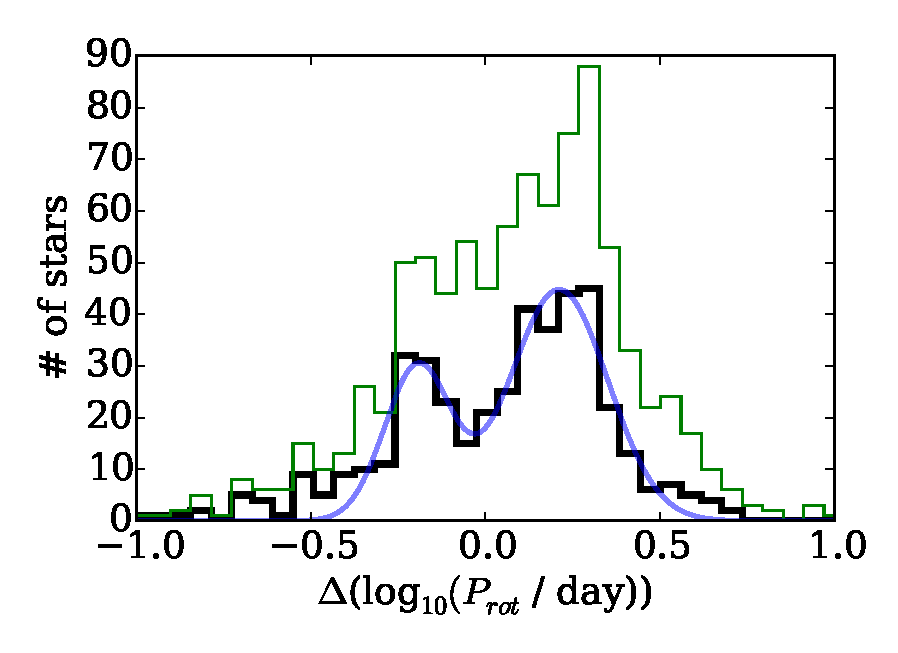
\includegraphics[width=3in]{davenport2016_fig4}
}
\caption{Left -- Figure 2 from \citet{davenport2017}, showing the absolute Gaia magnitude versus temperature for \Kepler stars with known rotation periods in the Gaia DR1 catalog. Sub-giant stars can be separated from main sequence targets using isochrone models (black solid \& dashed lines). Right -- Figure 4 from \citet{davenport2017}, showing the rotation period distribution relative to a 600 Myr ``gyrochrone'' before (green line) and after (black line) filtering out sub-giants. The bimodal distribution is apparent, and fit with a 2-Gaussian model (blue line).}
\label{fig:cmd}
\end{figure}

To determine which formation mechanism gives rise to the bimodal period distribution seen in the original \Kepler field, we must determine if the feature is only present in nearby stars. However, we must also rule out the unlikely possibility that the bimodality is due to some systematic error in the \Kepler data. Within each K2 campaign we will visually inspect the low-mass stars in the color--period space ($T_{eff}<4500$), as illustrated in Figure \ref{fig:bimodal} for the \citet{mcquillan2013} M dwarf sample. Since these coolest stars are only visible with \Kepler out to a few hundred pc, this will provide a test of the localization of the bimodality, using a small volume-limited sample. This test provides an important reality check against the period bimodality being due to the processing of the original \Kepler data itself. Since this initial nearby sample will probe the same close ($\sim$250 pc) volume as in \citet{mcquillan2013} and \citet{davenport2017}, we expect the period bimodality will appear up in most K2 fields for the M dwarfs centered around $P_{rot}=20$ days.



{\bf To reliably map the rotation period distribution as a function of distance we will match our final sample of K2 stars, and the original \Kepler rotation sample, to the upcoming data release from the Gaia mission} \citep{perryman2001}. With accurate parallaxes from Gaia for all \Kepler and K2 sources we will also be able to filter out subgiants and binary stars from our sample, leaving only main sequence stars. As \citet{davenport2017} showed, G dwarfs can only be used to detect the period bimodality if subgiants and binaries are filtered out.\citet{davenport2017} was able to do this for the \Kepler rotation period sample using the Gaia DR1 ``TGAS'' release that included astrometric data for nearby stars \citep{gaia_dr1}, as shown in Figure \ref{fig:cmd}. This reduced the \citet{mcquillan2014} rotation period sample of 33,000 sources down to the 440 brightest main sequence stars within $\sim$300 pc, roughly the same distance limit reached by the M dwarf-only sample. Studying the period distribution for G dwarfs is critical for including stars at further distances, and therefore sampling different star formation histories. {\bf With the April 2018 data release from Gaia we will be able to study rotation periods for G dwarfs in \Kepler and K2 out to $\sim$3 kpc.}


%JIM SAYS:  I hesitate to go here, b/c we open door to needing to determine kinematic ages, which will be a big fruitful and cool thing, but I don't want to personally do it if we don't have to...
% Gaia will also allow us to extend measurment made by \citet{mcquillan2013} in proper motion distributions, placing an additional constraint on the formation scenario.



Since the K2 campaign fields are spread across the entire ecliptic plane, rotation period data from fields with similar galactic latitudes can be combined to improve the sample size when searching for the bimodality as a function of distance. For example, C1, C3, C10, and C12 are near the North and South Galactic Caps, while C2, C7, and C13 straddle the Galactic Plane. The size scale over which the Milky Way's star formation history varies is unknown. In Andromeda significant variations in star formation histories are seen between 100 pc volumes, as well as large galaxy-wide trends \citep[e.g.][]{lewis2015}. We will therefore conduct our search for the period bimodality as a function of distance in each \Kepler/K2 pointing separately, as well in bins of galactic latitude.


The variation between K2 fields in the rotation period distribution will be most sensitive for the youngest stars, where stellar rotation evolution is most dramatic. If the young stars (short period bump in Figure \ref{fig:cmd}) were formed, for example, due to the passage of a Milky Way spiral arm, we would expect a shift in the peak of the rapid rotation distribution between fields ahead and behind the Sun along the direction of our Galactic orbit. Assuming a spiral arm pattern speed of $\Omega_{sp}= 25$ km s$^{-1}$ kpc$^{-1}$ \citep{dias2005,gerhard2011}, rapidly rotating stars at a distance of 1 kpc in opposing fields could have an age offset of $\sim$100 Myr, which should be detectable given a 10-20\% per-star age resolution for gyrochronology.


We will measure the strength of the bimodal feature by examining the period
distribution centered around a 600 Myr gyrochrone, as in Figure \ref{fig:cmd}.
By fitting multiple Gaussians to the period distribution in each bin of
galactic latitude and distance, we can empirically determine the significance
of the bimodality. The Bayesian Information Criterion allows us to
analytically determine if one or two (or more) Gaussian curves best represent
the rotation distribution in each spatial bin. If the bimodality is a generic
feature of angular momentum loss evolution, this two-Gaussian fit from
\citet{davenport2017} will be preferred for every latitude and distance bin.
If the bimodality is due to a localized age distribution of stars, we expect
the feature will disappear or shift as we go to further distances and sample
different star formation histories. %Other period bimodalities may be present
%given different star formation histories, but will not align to the 600 Myr
%gyrochrone.




%%%%%%%%%
\subsection{Mapping Ages in each Field}

Combining our catalog of rotation periods from K2 with the existing rotation
catalogs from Kepler will produce the largest set of rotation periods
currently available.
Using gyrochronology and other dating methods, we may be able to transform
these rotation periods into ages.

% Using a new technique being developed by CoI Angus, we will produce an
% improved age estimate for every star based on rotation values, photometric
% colors and galactic kinematics from Gaia proper motions.
% This age map may be used to infer the age distribution of stars within and
% across K2 fields.

As discussed above, the performance of the age-rotation relations for old
stars has been called into question in the last few years
\citep{angus2015,van-saders2016, Metcalfe2016}.
A simple straight-line model for rotational age does not reproduce the ages
predicted by asteroseismology for stars older than the Sun.
This phenomenon is attributed to a transitioning magnetic dynamo at a critical
Rossby number, $Ro$, of around the solar value \citep{van-saders2016}.
As rotation periods slow, $Ro$ decreases until it hits the critical value and
magnetic braking switches off: stars maintain their rotation period from that
point onward.
This feature of rotational evolution, if accurate, restricts the applicability
of gyrochronology to young, rapidly rotating stars.
A transitioning magnetic dynamo is supported by the existing data, however
these data are sparse~---~the analyses demonstrating the discrepancies were
conducted on a small number of main sequence, Solar-like oscillators observed
by Kepler in short cadence mode with detectable rotation periods: a sample
size of around 20.
% Furthermore, asteroseismology favors stars with low surface gravities since
% they show the largest amplitudes of oscillation and the majority of stars in
% this sample were slightly evolved.
A larger sample of old main sequence stars with precise ages is required to
confirm and further characterize the Rossby saturation mechanism introduced by
\citep{van-saders2016}.
However, old main sequence stars are difficult to age-date with any other
method than asteroseismology.
We propose use the age gradients in the kinematic properties of stars to
confirm the Rossby saturation effect.

There is evidence to suggest that stars in the Milky Way form in the thin disc
of the galaxy with relatively small vertical velocities and angular momenta
\citep[\eg][]{carlberg1985, edvardsson1993, freeman2002, bensby2004,
holmberg2007}.
These stars are slowly scattered via close encounters with other stars and
interactions with galactic spiral arms.
The more time passes, the more scattering events take place, and stars slowly
accumulate displacement and angular momentum in the z-direction, out of the
plane of the Milky Way.
Older stars can be identified in Gaia DR1 by integrating their orbits in the
potential of the Milky Way to convert their proper motions, positions and
parallaxes into vertical angular momenta, or actions.
The {\it dispersion} in vertical action for groups of stars reliably traces
age: an old population will have a larger dispersion in vertical action than a
young population.
Since most \Kepler\ and K2 stars will have positions, parallaxes and proper
motions measured by Gaia, we can calculate the vertical action dispersion for
groups of stars with various rotational properties.
Rapid rotators (young stars) should have smaller vertical action dispersions
than slow rotators (old stars).
We will calculate gyrochronological ages for all F, G and K dwarfs with
rotation periods and test these ages against their predicted kinematic ages.
In this way we will test the gyrochronology relations and, in particular,
confirm whether rotation continues to be a good age proxy at late ages, \ie\
does the \citet{barnes2003} model or a \citet{van-saders2016} model provide a
better description of the data?
{\bf We propose to use the relationship between vertical action and age to
test the gyrochronology relations at late ages.}

The intersection between Gaia and \Kepler/K2 rotators provides another test of
the age-rotation relations.
Over 13,000 comoving pairs of stars were identified in the first Gaia data
release by \citet{Oh2016}.
Several hundred of these pairs fall in the \Kepler/K2 footprint.
If these comoving stars are coeval, their rotation periods should predict the
same gyrochronological age.
The dispersion in rotational-age, predicted from the rotation periods of
coeval groups of stars will reveal the fundamental uncertainty in the
gyrochronology relations.
We have secured 5 nights on the ModSpec spectrograph on the Hiltner 2.4m
telescope at MDM observatory, to obtain radial velocities for the comoving
pair candidates in the \Kepler\ field.
A previous observing run established that around 80\% of the \citet{Oh2016}
comoving pairs, identified from 2-dimensional proper motions, have radial
velocities consistent with being comoving.
We expect to find this same low false-positive rate for the comoving pair
candidates in the \Kepler\ field.

Having established whether the \citet{barnes2003} or \citet{van-saders2016}
model is more appropriate for describing the rotational evolution of stars, we
will apply a new dating method (called {\tt chronometer}) that combines
multiple age indicators in order to produce an age map of the K2 sky.
{\tt chronometer} extends isochrone fitting by simultaneously fitting an
age-rotation relation and a age-velocity dispersion relation to stars with
photometric colors, rotation periods and Gaia proper motions.
It combines the information available from these three dating techniques, thus
providing more accurate ages than any one of the techniques alone.
Figure \ref{fig:chrono} demonstrates how combining multiple dating methods can
improve both the precision and accuracy of an age measurement.
% {\tt chronometer} combines gyrochronology, stellar evolutionary tracks,
% asteroseismology and galactic kinematics by jointly inferring the parameters
% of the three different models.

\begin{figure}[!ht]
\centering
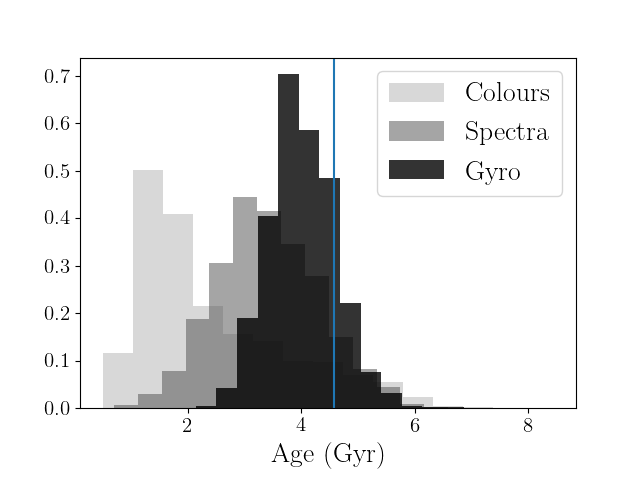
\includegraphics[width=4in]{all_hist_working.png}
\caption{A preliminary demonstration of the power of rotation for age
    inference, created using {\tt chronometer}.
    The palest gray histogram shows the probability distribution over ages
    obtained for the Sun at 10 parsecs using only J, H and K band colors.
    The darker gray histogram shows the age posterior for the Sun at 10
    parsecs using colors and spectroscopic information ($T_{\mathrm{eff}}$,
    $\log(g)$ and $[Fe/H]$).
    The darkest gray histogram shows the age posterior when colors,
    spectroscopic information and a rotation period used to infer the age of
    the Sun at 10 parsecs.
    This is a preliminary plot with no kinematic information and just three
    stars.
    The final model will contain several thousand stars and kinematic
    information so will be even more powerful than this.
}
\label{fig:chrono}
\end{figure}

% The unique aspect of our analysis is to combine inference over ages with
% calibration of the free parameters in the gyrochronology and vertical
% action-age relations.
% The global parameters, the parameters of the gyrochronology relation and the
% age-velocity dispersion relation will be inferred separately from the
% individual parameters of each star.
% This analysis involves a large number of free parameters: several global
% parameters and five individual parameters per star.
% Inferring the ages of one thousand stars will require sampling the posterior
% probability density functions of five thousand and four parameters.
% This sounds like a large number but we can use conditional independence to
% break this problem down and apply Gibbs sampling to increase tractability.
% This means we will only explore the PDFs of a maximum of five parameters at a
% time.

% In classical isochrone fitting, one might calculate the probability of age
% $A$, mass $M$, \feh, distance $D$ and extinction \av, given a set of
% apparent magnitudes in different filters, \eg\ $M_V$, $M_J$ and $M_K$.
% % This can be written
% % \begin{eqnarray}
% %     &&p(A, M, [Fe/H], D, A_v | M_V, M_J, M_K) \\ \nonumber
% %     \propto &&p(M_v, M_J, M_K | A, M, [Fe/H], D, A_v) \\ \nonumber
% %     &&p(A)p(M)p([Fe/H])p(D)p(A_v).
% % \end{eqnarray}
% There are no free parameters in the model here --- the model is entirely
% determined by physics and does not need to be calibrated further.
% A suitable set of stellar evolution models would be selected for the
% inference, for example the Dartmouth models
% {\bf Ruth: add citation}.
% Similarly, in classical gyrochronology, one might calculate the probability of
% age given rotation period and $B-V$ colour,
% % \begin{equation}
% %     p(A | P_{rot}, B-V) \propto p(P_{rot}, B-V | A)p(A)
% % \end{equation}
% In a gyrochronology model however, our understanding of the physics is
% incomplete and some free parameters must be calibrated.
% In the \citet{barnes2003} gyrochronology parameterisation, $A =
% P_{\mathrm{rot}}^{1/n} - (B-V-0.4)^{b/n}$, these free parameters are $a$, $b$
% and $n$.
% During a calibration exercise, the observables, $A$, $P_{rot}$ and $B-V$ will
% be known and the parameters, $a$, $b$ and $n$ will be inferred.
% % \begin{equation}
% %     p(a, b, n | \{A\}, \{P_{rot}\}, \{B-V\}) \propto \{p(A\}, \{P_{rot}\},
% %     \{B-V\} | a, b, n) p(a)p(b)p(n).
% % \end{equation}
% The age-velocity dispersion relation also has free parameters that must be
% calibrated using observations, for example the coefficient of increasing
% dispersion.

% The unique aspect of our analysis is to combine inference over ages with
% calibration of the free parameters in the gyrochronology and vertical
% action-age relations.
% The global parameters, the parameters of the gyrochronology relation and the
% age-velocity dispersion relation will be inferred separately from the
% individual parameters of each star.
% This inference problem involves a lot of free parameters: at least four global
% parameters and five parameters per star.
% Inferring the ages of one thousand stars will require sampling the posterior
% probability density functions of five thousand and four parameters.
% % \begin{eqnarray}
% %     &&p(\{A\}, \{M\}, \{[Fe/H]\}, \{D\}, \{A_v\}, a, b, n, \alpha, \beta|
% %     \{M_V\}, \{M_J\}, \{M_K\}, \{P_{rot}\}, \{B-V\}, \{J_z\}) \\ \nonumber
% %     \propto &&p(\{M_v\}, \{M_J\}, \{M_K\}, \{P_{rot}\},
% %     \{B-V\}, \{J_z\} | \{A\}, \{M\}, \{[Fe/H]\}, \{D\}, \{A_v\}, a, b, n,
% %     \alpha, \beta) \\ \nonumber
% %     &&p(A, M, [Fe/H], D, A_v, a, b, n, \alpha, \beta).
% % \end{eqnarray}
% This sounds like a large number but we can use conditional independence to
% break this problem down and apply Gibbs sampling to increase tractability.
% This means we will only explore the PDFs of a maximum of five parameters at a
% time.
% down further into the
% following:
% \begin{eqnarray}
%     &&p(\{A\}, \{M\}, \{[Fe/H]\}, \{D\}, \{A_v\}, a, b, n, \alpha, \beta|
%     M_V, M_J, M_K,
%     \{P_{rot}\}, \{B-V\}, \{J_z\}) \\  \nonumber
%     \propto &&p(\{M_v\}, \{M_J\}, \{M_K\} | \{A\}, \{M\}, \{[Fe/H]\}, \{D\},
%     \{A_v\})
%     p(A)p(M)p([Fe/H])p(D)p(A_v) \\ \nonumber
%     &&p(\{P_{rot}\}, \{B-V\}, a, b, n | A)p(a)p(b)p(n) \\ \nonumber
%     &&p(\{J_z\}, \alpha, \beta | \{A\}) p(\alpha)p(\beta).
% \end{eqnarray}
% Informally, the structure of this inference procedure can be written as
% \begin{eqnarray}
%     &&p(\mathrm{Ages~\&~other~parameters}|\mathrm{observables}) \\
%     \propto &&\mathcal{L}_{\mathrm{isochronal~age}} \times
%     \mathcal{L}_{\mathrm{gyro~age}} \times
%     \mathcal{L}_{\mathrm{kinematic~age}} \\
%     && \times p(\mathrm{Ages~\&~other~parameters})
% \end{eqnarray}.
% We can multiply the likelihoods together by making the assumption that the
% probabilities are conditionally independent, \ie\ a gyrochronology age depends
% only on rotation period and colour, not proper motion, for example.
% In reality this assumption is not valid because gyrochronology ages do depend
% on \logg, \teff\ and \feh.

% This is essentially an extension of the period bimodality work (if it's an age
% effect), but to create a detailed map of the ages of these field stars at a
% range of galactic latitudes in the 17 pencil-beams available from K2.
% combining with the periods from Kepler, will be even better.
% Ultimately we'd like to compare to the age distributions in simulations of
% these fields from TRILEGAL, and from other age indicators (asteroseismology,
% flare ages, etc).



%%%%%%%%%%%%%%%%%%%
\section{Team Qualifications}
PI Davenport has used \Kepler to conduct the largest survey to-date of stellar activity from flares, as well as multiple investigations of starspots and their evolution with time using \Kepler data. From these studies, Davenport has developed an age model for flare activity that will be directly comparable to the ages and starspot amplitudes derived from this study. He also recently discovered the rotation period bimodality first noted with \Kepler M dwarfs by \citet{mcquillan2013} extends to G and K dwarf stars \citep{davenport2017}.
Davenport previously collaborated on NASA ADP grant NNX09AC77G to characterize NIR variability using the 2MASS Calibration Scan Point Source Working Database \citep{davenport2012,davenport2015a}.
He has mentored numerous students on projects using \Kepler data, resulting in student-led publications such as the flare activity of a unique M dwarf binary system GJ 1245AB \citep{lurie2015}, and exploring the poorly understood origins of wide binary stars through stellar rotation (R. Clarke in prep). He will manage the overall project, detect and remove short period variability from flares in the light curves, supervise the initial periodic signal detection using Lomb-Scargle methods, and lead the investigation and publication on the nature of the bimodal period distribution.

Co-I Angus is an expert in the extraction of periodic signals from \Kepler
data using Gaussian Processes \citep{angus2016c} and other cutting-edge
statistical techniques.
She is the author of tools for generating Systematics-Insensitive Periodograms
for K2 data \citep{angus2016}, as well as new gyrochronology calibrations
using \Kepler asteroseismic targets \citep{angus2015}.
She will lead the effort to measure and publish the catalog of rotation
periods for all K2 sources, recalibrate the gyrochronology relations using the
rotation periods of \Kepler and K2 stars observed by Gaia and measure ages for
field stars using the {\tt chronometer} Python code.

Covey
wrote white paper of stellar age dating techniques  for decadal survey \citep{covey2010white}
expertise working with \Kepler and K2 data to search for periods \citep{douglas2016,covey2016}

Kipping
has developed analytical models for rotational modulations in stellar light curves \citep{kipping2012}, and recently used Gaussian Processes to detrend systematics and search for periodicities from MOST data of Proxima Centauri \citep{kippingmost}. He will provide expertise in advanced statistical techniques to detrend and study the K2 data to help Co-I Angus in her period detection and validation efforts.

Agueros
ongoing study of rotation in clusters from both the ground \citep{agueros2011} and with \Kepler/K2 \citet{douglas2016,douglas2017,nunez2017}.




%%%%%%%%%%%%%%%%%%%
\section{Relevance to NASA Programs}
history of MWY, age of planet systems, TESS



%%%%%%%%%%%%%%%%%%%
\section{Plan of Work}
{\bf Year 1:} Produce a catalog of K2 rotation periods. Perform exploratory
analysis of these data, including a search for extended bimodality.
Produce a newly calibrated relation between rotation and age,
based on the kinematics of \Kepler and K2 stars with Gaia proper motions and
parallaxes.
\\
{\bf Year 2:} Produce an age map of the K2 sky using the newly developed 
{\tt chronometer} code.
Explore the implications of this age map for galactic archaeology.


\clearpage
%\pagestyle{empty}

\bibliography{references}


\end{document}
